\centerline{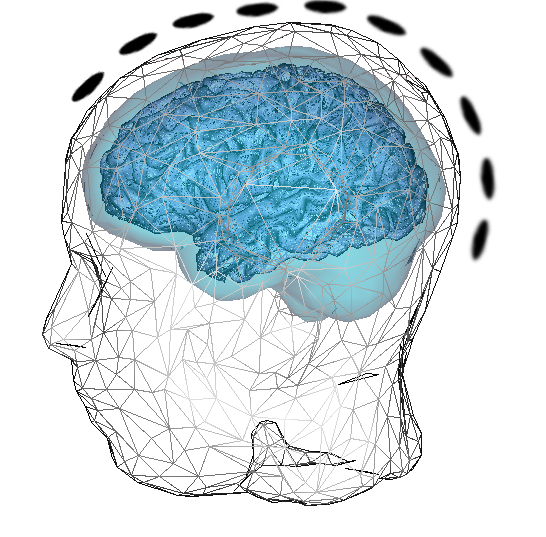
\includegraphics[height=9cm]{surf3.png}}

\noindent
The forward problem consists in simulating the electric potential (EEG) and magnetic fields (MEG) on the sensors due to electrical sources within the brain.

\centerline{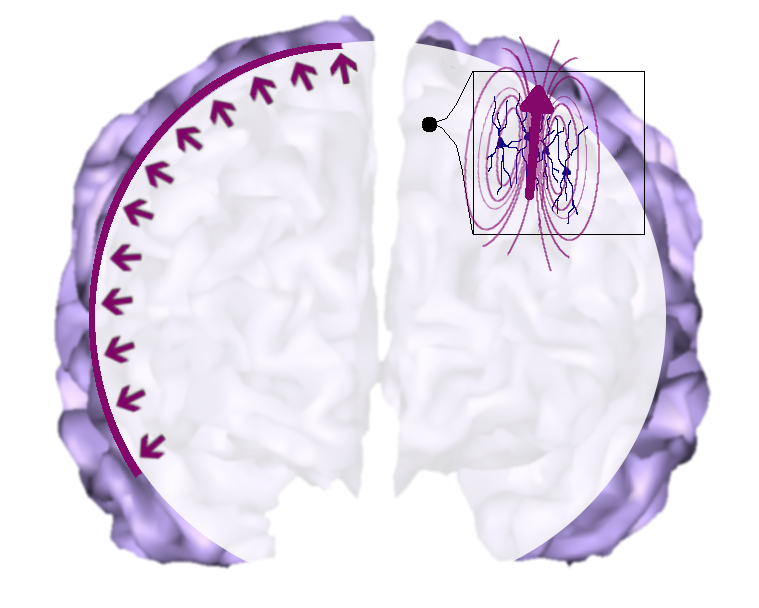
\includegraphics[height=10cm]{dipole.png}}

\noindent
\underline{Step 1}~: the potential is computed on \textbf{all surfaces } of the head model (scalp, outer skull and inner skull for a three-layer model).  Let $\mathbf{X}$ contain the values of the potential on the discretized surfaces, as well as the values of the normal current. The Boundary Element Method leads to a linear system:
\[
    \mathbf{HeadMat} . \mathbf{X} = \mathbf{SourceMat}
\]
See sections \ref{sect: command assemble HeadMat}, \ref{sect: command assemble SourceMat} and \ref{sect: command invert HeadMat}.

\medskip

\noindent
\underline{Step 2}~: the matrices relating the head model surfaces and the sensor data must be computed. These are different for EEG and for MEG.\\
\\
For EEG, the potential is interpolated from the surface discretization points to the sensor positions through a simple linear transformation~:\\
\[
    \left[ \mbox{potential at sensors} \right] =
    \left[ \mbox{interpolation matrix} \right] \times \left[ \mbox{potential at interfaces} \right] \mbox{in the case of EEG.}
\]
For MEG, the Biot and Savart equation allows to identify two contributions to the magnetic field: one which comes directly from the sources, and an ohmic contribution which comes from the volume conductor. 
Hence two linear transformations must be computed, one from the source locations  to MEG sensors, the other from the head model interfaces to the MEG sensors.\\

\noindent
See section \ref{sect: command assemble sensors}.

 
\medskip

\noindent
\underline{Step 3}~: the matrix relating the sources (at fixed positions and orientations) to the sensors is now ready to be computed (section \ref{sect: command gain}). This matrix is called  the \textbf{gain matrix} and is denoted  $\mathbf{G}$. The gain matrix is then applied to the source activation to simulate the forward problem  (section
\ref{sect: command direct}).
